% ==============================
% Chapter 4
% ==============================

\begin{center}
    \section*{\fontsize{20}{20}\selectfont Chapter 4}
\end{center}
\vspace{10mm}

\section{Implementation and Result Analysis}

This chapter will try to elaborate on the implementation details and evaluation of the our proposed pose-based autism behavior classification framework. The analysis will be carried out by considering traditional machine learning and deep learning techniques on short video segments of 3-4 seconds in length. The key side of this chapter will be to understand and analyze the performance of the models on the preprocessed data and evaluate them on different parameters such as generalization, temporal modeling, and interpretability of results and aslo  traditional classification performance and existing approaches.

% ==============================
\subsection{Environment Setup}

All the experiments are employed through Python-based Machine Learning and Deep Learning techniques. The pose extraction method is employed by MediaPipe Pose. The classical models are employed using the scikit-learn library and the Deep Learning models are employed by using the very popular TensorFlow and Keras. The code is written in the google colab with internal T4 GPU to support the processings and also the sequence based learning process which is really cruicial for the video based experiments like ours. For reproducibility, the random seeds and software versions were kept the same across all the experiments pre purposedly.


% ==============================
\subsection{Data Preprocessing}

This step converts the raw behavioral videos into a more structured and numerical form that can be used for machine learning and deep learning models. The process begins from the extraction of frames from the videos and then followed by the extraction of pose landmarks and the normalization of the timing before starting the feature set.

\subsubsection{Video Frame Extraction}

The raw videos of the certain behaviors is broken down into frames using OpenCV. The videos got different resolutions, for this reason frames are resized to a fixed width while maintaining the aspect ratio.  

\subsubsection{Pose Landmark Extraction}

For each frame, the Human pose is extracted using the MediaPipe Pose library. The library has 33 key points on the body and they are the head, shoulders, elbows, wrists, hips, knees, ankles, and more. For each of these points, three values are recorded in the x and y coordinates as well as the visibility score on the confidence of the pose extraction.

So,each frame is represented as 99 dimensional vector with each dimension to one of the 33 points on the body and the three values for each point. If the pose extraction for a frame fails, a zero vector will be used to maintain the sequence.

\subsubsection{Temporal Sequence Normalization}
The videos that we have collected have different lengths and different frames in each video. For this reason, we had to standardize all the pose sequences to a uniform length of 30 frames. We achieved this in the following way like if the sequence is lower than 30 frames, we jsut simply repeat the last detected frame until we reach our desired 30 frames. On the other hand, if the sequence is greater than 30 frames, we use the method even sampling to pick frames that are representing type of the entire range of the video.

\subsubsection{Constructing Features for Classical Models}

To use classic machine learning classifiers, we have transformed each pose sequence to a fixed-size feature vector. We have computed several statistical descriptors for each pose landmark coordinate and they are the mean, standard deviation, minimum, maximum respectively.

\begin{figure}[htbp]
\centering
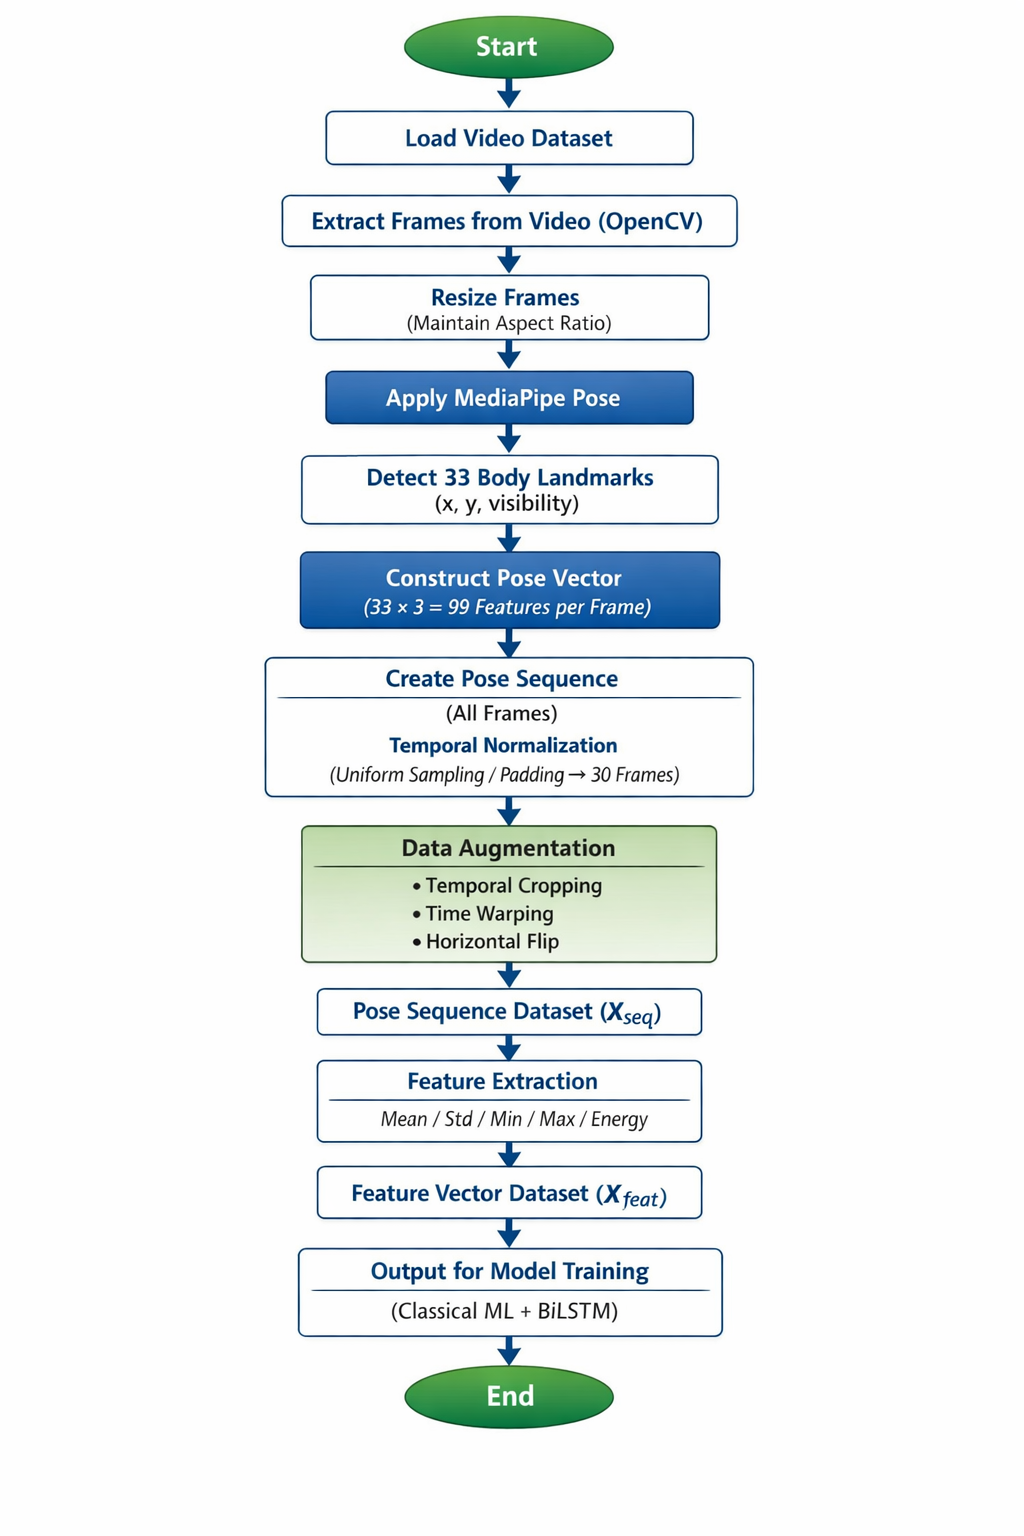
\includegraphics[width=0.8\textwidth]{image/data_preprocessing.png}
\caption{Data Preprocessing Steps}
\label{fig:Data_Preprocessing}
\end{figure}

In the Figure \ref{fig:Data_Preprocessing}, we show the step and stage involved with preprocessing video data. At first, we get the frames from the videos. Then, we use the MediaPipe Pose model to get 33 body keypoints per frame (x, y, visibility), thus having 99 features per frame. Because of the fact that videos differ in length, we try make sure that all videos have 30 frames by either padding or reducing the number of frames.Also, to make sure that our neural networks generalize well, we use some techniques such as sequence cropping, time warping and horizontal flips. Consequenctly, we form two different kinds of datasets: raw pose sequences for deep learning analysis and statistical features for classical ML models.

% ==============================
\subsection{Feature Relationships}

\begin{figure}[htbp]
\centering
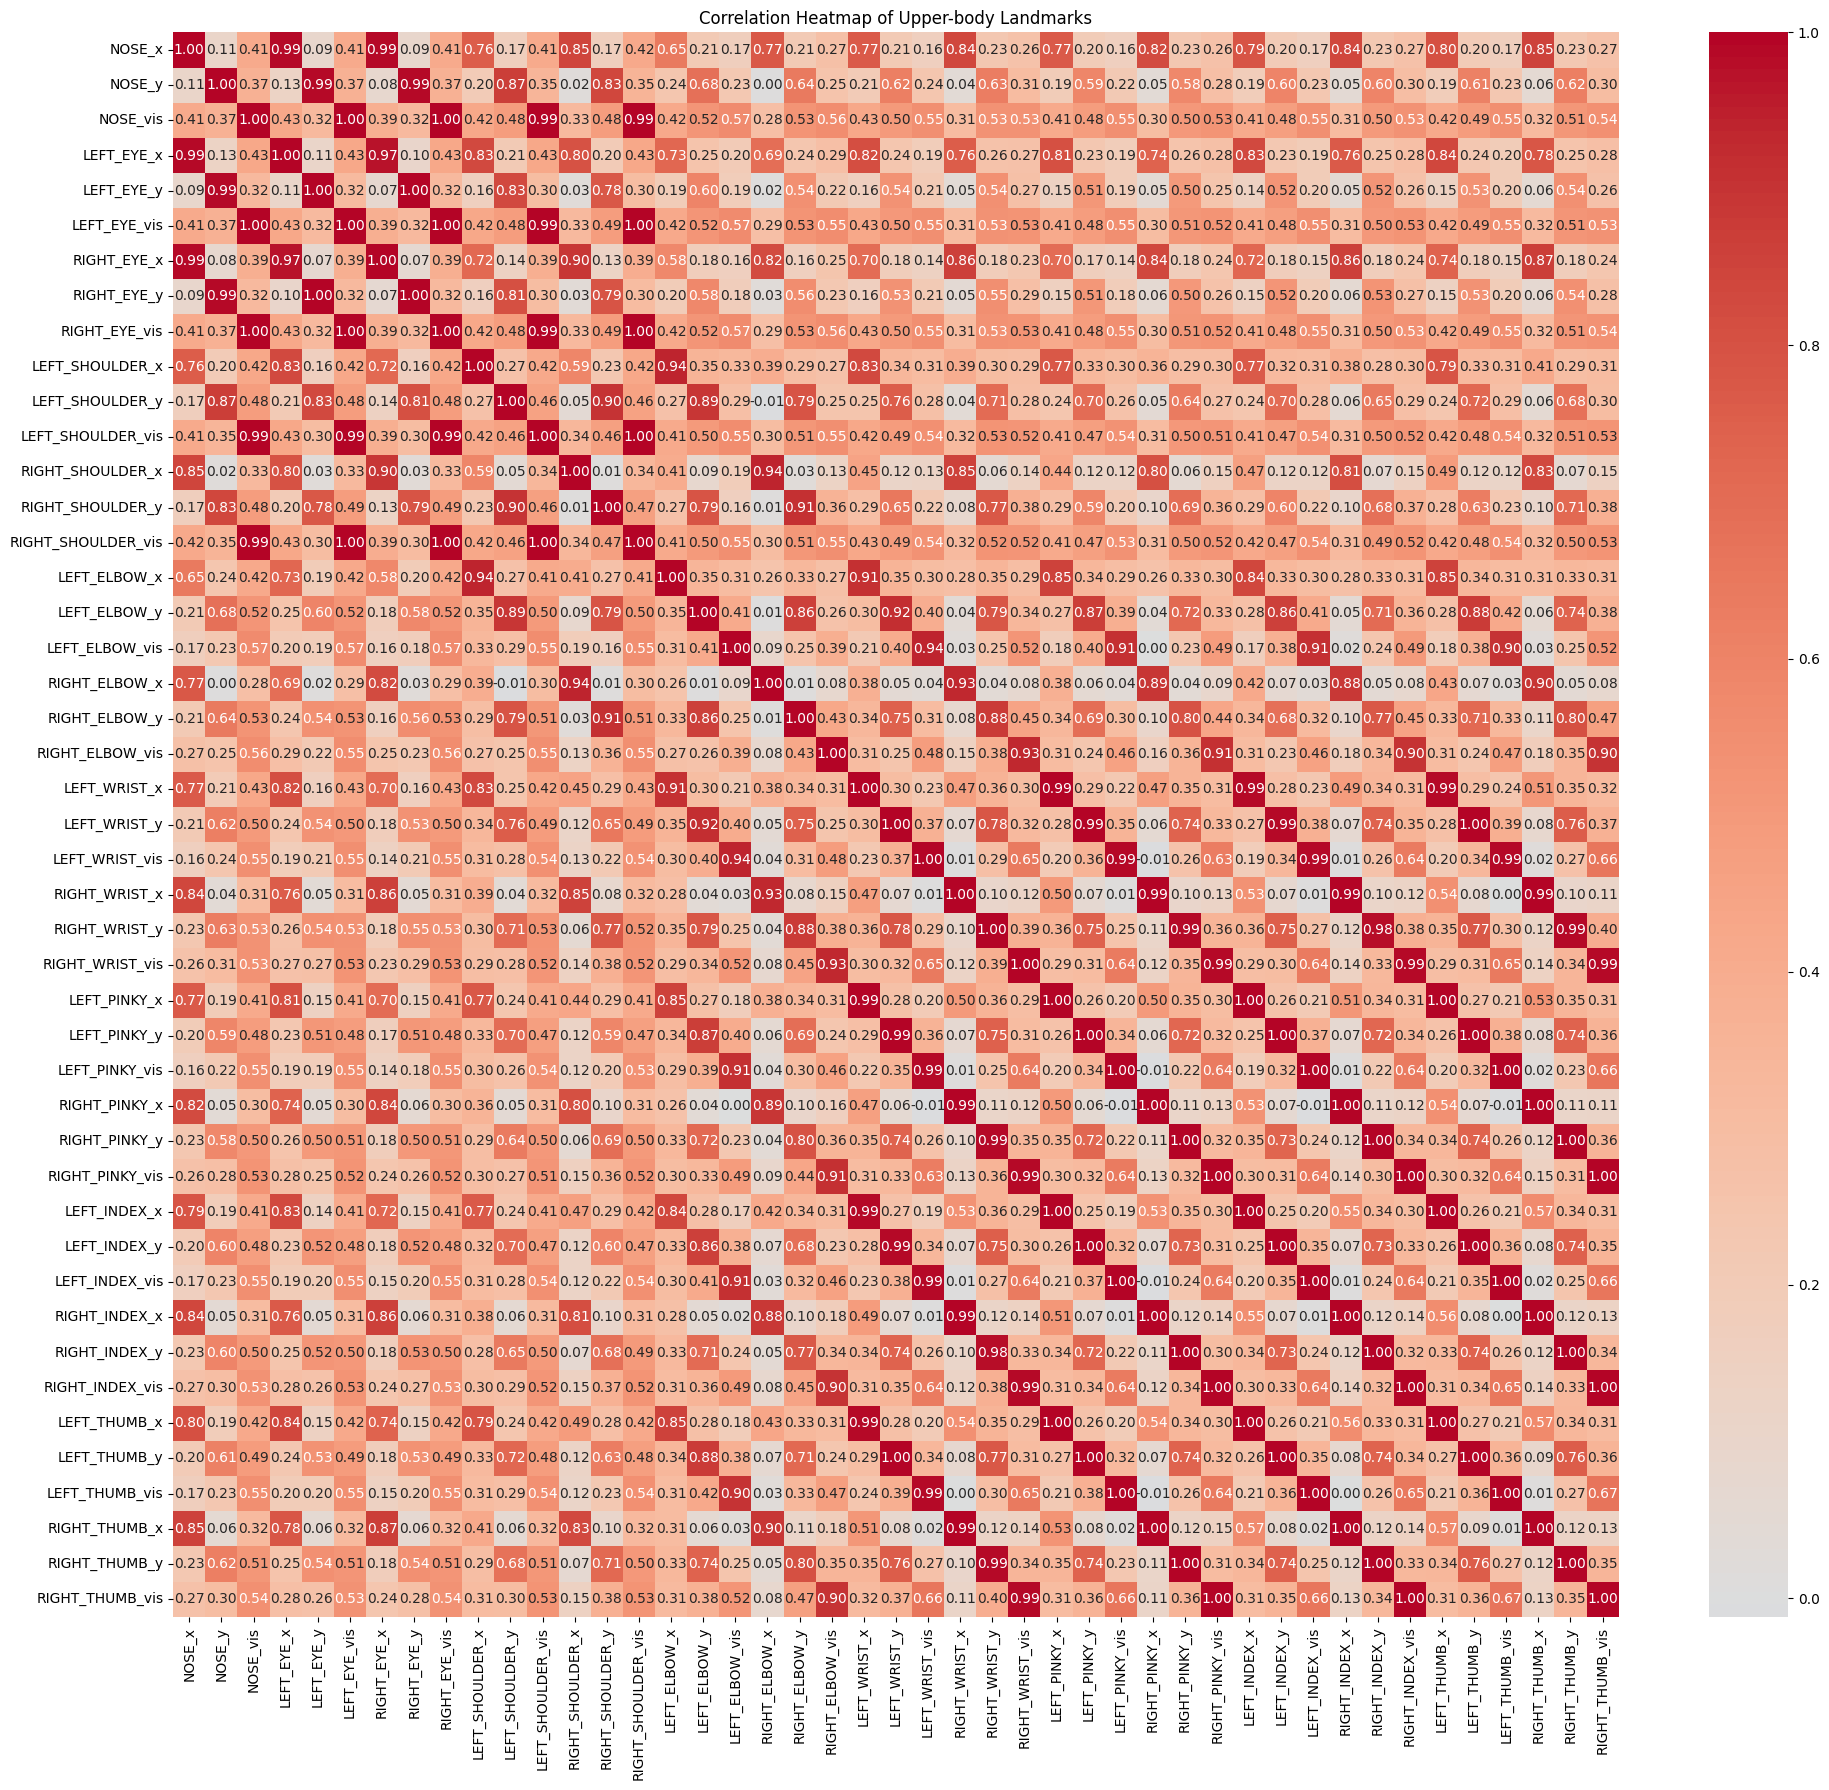
\includegraphics[width=0.8\textwidth]{image/correlation_heatmap.png}
\caption{Correlation heatmap of upper-body pose landmark features.}
\label{fig:corr_upper}
\end{figure}


In the Figure \ref{fig:corr_upper}, upper body landmark of skeletal frames correlation has been tried to show as a heatmap. The heatmap clearly is dark or darked red where only trademak body landmarks statistical features is highly correlated to other. For example from the heatmap we can clearly see with the right wrist, right thumb is heavily correlated by dark red which may indicated a certain correlation with hand flapping and finger clipping and onwards.

% ==============================
\subsection{Model Implementation}

We have used both classical machine learning model and deep learning model for our thesis as detailed below:

\subsubsection{Machine Learning Models}
A number of conventional machine learning architectures are implemented and they are Random Forest, Support Vector Machine, Logistic Regression, K-Nearest Neighbors, and Gradient Boosting respectively. These model architectures are trained on statistical features that have been learned from the pose data. In order to make the system more robust, ensemble methods with hard voting and soft voting have also been considered.

\subsubsection{Deep Learning Model}
To demonstrate the temporal dependencies properly, a Bi-Directional Long Short-Term Memory (BiLSTM) network has also been trained directly on the normalized pose sequences. The BiLSTM network views the sequences both forward and backward, thus allowing it to learn short repeating patterns very well which is very important for our thesis. To avoid overfitting in the model, dropout and early stopping are applied. Class weighting have also been used to remove class imbalance.
Also later, BiGRU has been introduced for computational feasibility and less gating and CNN for combining one-dimensional convolutional layers with bidirectional LSTM layers.

% ==============================
\subsection{Evaluation Metrics}

Performance metrics are calculated using standard multiclass metrics which are commonly announced as accuracy, precision, recall, and F1 score. Confusion matrices are used to gain further insight informations for the prediction split. Also, we compute One-vs-Rest ROC curves and the corresponding AUC values for the BiLSTM. When using conventional machine learning models, we relied on five-fold stratified cross-validation. Also,confusion matrix and ROC AUC curves have also been generated for these machine learning models too.
\begin{figure}[htbp]
\centering
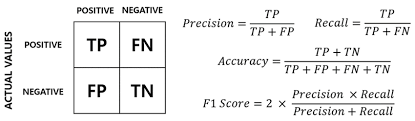
\includegraphics[width=0.8\textwidth]{image/f1.png}
\caption{Formula of Precision, Recall, Accuracy, and F1 score}
\label{fig:Formula of Precision, Recall, Accuracy, and F1 score}
\end{figure}


% ==============================
\subsection{Performance Analysis}

We have evaluated our project from two perspectives. The first one is from the view of traditional and classical machine learning models which work only features like 33 landmarks of human skeleton from media pose and the later is the deep learning model for exploiting the temporal dependency of frame to frame of pose sequences to accurately evaluate whether our work is generation results or not.

\subsubsection{Traditional Models Performance Analysis}

In the conventional models, we first implemented a five-fold cross-validation to assess the performance of the pose-based feature representation so that the statistical features can be extracted.

The plotting below compares the testing accuracies of our traditional models used in this thesis from 5 fold validation and 70\% training, 15\% testing and 15\% validation perspective.

\begin{table}[htbp]
\centering
\caption{Model Performance Comparison}
\label{tab:model_comparison_after_split}
\begin{tabular}{l c c c}
\hline
\textbf{Model} & \textbf{Validation Acc} & \textbf{Test Acc} & \textbf{Log Loss} \\
\hline
Random Forest & 0.8762 & 0.8952 & 0.4341 \\
SVM & 0.4667 & 0.5143 & 1.2620 \\
Logistic Regression & 0.7524 & 0.7905 & 1.2118 \\
KNN & 0.5810 & 0.6286 & 3.9598 \\
Gradient Boosting & 0.8571 & 0.8667 & 0.5189 \\
Soft Voting & 0.8190 & 0.8286 & 0.4726 \\
Hard Voting & 0.8762 & 0.8952 & N/A \\
\hline
\end{tabular}
\end{table}

From this table \ref{tab:model_comparison_after_split} and from the figure \ref{fig:split_trad} it is cleary evident that the winner in terms of accuracy is the Random Forest Classifier and Hard Voting both having 89.5\% test accuracy. However, the problem with these models is that they are more overfitted compared to the Gradient Boosting model since their validation accuracies are 2 percentage points lower than their testing accuracies. In the case of the Gradient Boosting Classifier, there is virtually no difference between its validation and test accuracy, which is 85.7\% and 86.7\%, respectively, and its log loss is constant at 0.5189. This suggests that the model has been trained to make consistent probability predictions. As for the Random Forest Classifier, its test accuracy is higher by 1.9 percentage points than its validation accuracy, but the difference is not significant.



\begin{figure}[htbp]
\centering
\includegraphics[width=0.8\textwidth]{image/5_fold_trad.png}
\caption{Classical Model Accuracy after 5 fold validation with Ensembel Method}
\label{fig:5_fold_trad}
\end{figure}

\begin{figure}[htbp]
\centering
\includegraphics[width=0.8\textwidth]{image/split_trad.png}
\caption{Classical Model Accuracy after 70\% training, 15\% testing and 15\% validating with Ensembel Method}
\label{fig:split_trad}
\end{figure}

So this figure \ref{fig:5_fold_trad} is the 5-fold cross-validation accuracy, sorted from worst to best. SVM is at the bottom again barely 48\% which is basically useless. KNN follows at 69\%, still weak. After that Logistic Regression at 86.3\% which is very decent but it is also nothing special but mean time worth it. Gradient Boosting and Soft Voting tie at 89.4\% — solid and consistent. But the real stars are Hard Voting at 92.4\% and Random Forest at 92.6\%, sitting at the top and almost identical. What matter in here is that in cross-val, there's no overfitting trick — every fold is unseen. So Random Forest and Hard Voting genuinely generalize well across different splits. Gradient Boosting still looks stable, but it's now 3\% behind the leaders. So the bottom line is that Random Forest and Hard Voting are your safest bets if the reliability is wanted across different data cuts.

Hardvoting Ensemble was done here combining Random forest and Gradient Boosting and to break the tie Random forest was given the upper vote. SoftVoting was initiated by predictions from three classifers random forest, gradient boosting and logistic regression as the average performer. Random forest always performed exellent as it uses decision trees and Gradient boosting followed side by side as it sequentially boosts the weak learner. Logistic Regression worked as a polynomial decision boundry baseline and the bad performing SVM fitted the pose derived statistical features poorly. KNN got sensitive to feature scaling and local patterns of distances so it performed bad.

Looking at both the train/test split and the 5-fold cross-validation, Random Forest and Hard Voting consistently lead — hitting 89.5\% on test and 92.6\% in CV, with minimal overfitting signs. Gradient Boosting is the most stable: its test accuracy (86.7\%) almost matches CV (89.4\%), and its low, steady log loss (0.52) proves excellent calibration. In contrast, SVM fails everywhere (51\% test, 48\% CV), while KNN struggles with wild log loss (3.96). So if you want pure accuracy, pick Random Forest or Hard Voting. But if you need reliable probabilities and generalization, Gradient Boosting is the safer, more honest choice.


As we can also see, Gradient Boosting generalizes more stably later in the figure \ref{fig:rf_vs_gb_loss}, so it is sane that we chose Graident Boosting as our baseline model for our thesis.Gradient Boosting is optimized step by step by calculating gradients with respect to the features and gradually decreases the learning reate and finally tends towards a steady minimum of the log-loss with is crucial for classification work like ours.Hence, Gradient Boosting is selected as the main classical baseline model for our thesis although it has less accuracy than Random forest as a traditional model which works for statical features of our dataset.

Following we will analize the classification performance of Gradient Boosting.


\paragraph{Classification Report} : 

From Table~\ref{tab:gb_classwise},What actually stands out is that the model absolutely loves Spinning — it catches every single one (recall of 1.00). Tilting and Head Touching are also solid, especially Head Touching — when it says it's head touching, it's right 94\% of the time. But then there's Hand Flapping. That's the problem child. Recall sits at just 0.76, meaning the model misses nearly a quarter of actual hand flapping episodes. If you're tracking this behavior closely, that's a real issue. Because finger clipping and hand flapping can be very hard to differentiate even from the naked human eye.Finger Clipping sits right in the middle — nothing amazing, nothing terrible. Everything balanced at 0.81.
So the bottom line here is that the model works great for spinning and tilting, but don't trust it blindly for hand flapping. Overall accuracy (0.87) sounds nice.

\begin{table}[htbp]
\centering
\caption{Class-wise Performance of Gradient Boosting Model}
\label{tab:gb_classwise}
\begin{tabular}{l c c c c}
\hline
\textbf{Behavior} & \textbf{Precision} & \textbf{Recall} & \textbf{F1-score} & \textbf{Support} \\
\hline
Finger Clipping & 0.81 & 0.81 & 0.81 & 21 \\
Hand Flapping & 0.84 & 0.76 & 0.80 & 21 \\
Head Touching & 0.94 & 0.81 & 0.87 & 21 \\
Spinning & 0.84 & 1.00 & 0.91 & 21 \\
Tilting & 0.91 & 0.95 & 0.93 & 21 \\
\hline
\multicolumn{4}{r}{\textbf{Accuracy}} & 0.87 \\
\multicolumn{4}{r}{\textbf{Macro Avg}} & 0.86 \\
\multicolumn{4}{r}{\textbf{Weighted Avg}} & 0.86 \\
\hline
\end{tabular}
\end{table}

\paragraph{Confusion Matrix for Gradient Boosting} :

Looking at the confusion matrix in the figure \ref{fig:gradient_confusion} for Gradient Boosting, the story from Table~\ref{tab:gb_classwise} plays out clearly. Spinning and Tilting are nearly flawless — only 1 miss each, and those are just confused with each other. That's fine.

Head Touching gets 17 right, but messes up 3 times: 1 called finger clipping, 1 hand flapping, 1 spinning. Not terrible. Finger clipping gets 17 correct, but slips into hand flapping twice and head touching twice — some confusion but manageable. Because finger cliping and hand flapping are hard to differentiate even to the human eye. Then there's Hand Flapping. Only 16 correct out of 21. It gets mislabeled as finger clipping (3 times) and head touching (once). So the bottom line here is that the matrix confirms the model is great for spinning/tilting, shaky for hand flapping which is explainable.

\begin{figure}[htbp]
\centering
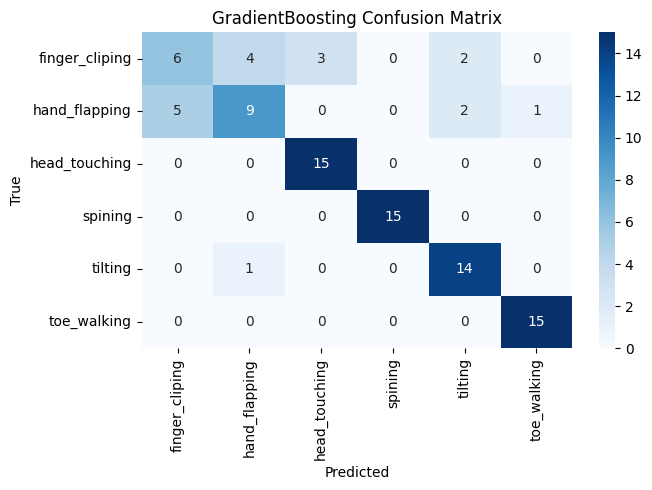
\includegraphics[width=0.8\textwidth]{image/gradient_boosting_confusion_matrix.png}
\caption{gradient boosting confusion matrix}
\label{fig:gradient_confusion}
\end{figure}



% ==============================
\subsubsection{Deep Learning Models Performance Analysis}


We had to implement the Deep Learning Models to exploit the temporal dependencies of frame to frame of pose sequences to evalute our work whether its generating the acutal results. Following are the detailed representations.

\begin{table}[htbp]
\centering
\caption{Final Comparison of Deep Learning Models (using 5-Fold Cross Validation)}
\label{tab:dl_model_comparison_5_fold}
\begin{tabular}{l c c c}
\hline
\textbf{Model} & \textbf{Mean Accuracy} & \textbf{Std Dev} & \textbf{Mean Loss} \\
\hline
BiLSTM & 0.7971 $\pm$ 0.0567 & 0.0567 & 0.5917 \\
BiGRU & 0.8343 $\pm$ 0.0330 & 0.0330 & 0.5192 \\
CNN-BiLSTM & 0.8100 $\pm$ 0.0469 & 0.0469 & 0.6225 \\
\hline
\end{tabular}
\end{table}

From Table~\ref{tab:dl_model_comparison_5_fold}, BiGRU  hits the highest mean accuracy (83.4\%) and the lowest loss (0.52), which tells you it's making confident, correct predictions. But here's what really matters: look at that standard deviation. BiGRU's is 0.033, the smallest of the three. That means it's not just good — it's consistent across all five folds. No wild swings.

CNN-BiLSTM sits in the middle on accuracy (81.0\%), but its loss is the highest (0.6225) — meaning when it's wrong, it's confidently wrong. But later seen in the validation log loss plotting \ref{fig:rf_vs_gb_loss} its generalization is reliable.

BiLSTM comes at 79.7\%, but the standard deviation is much larger (0.0567). So it's more hit or miss. Some folds it does okay, others it struggles. That's risky if reliability is needed.



\begin{table}[htbp]
\centering
\caption{Final Summary of All Models using 70\% training, 15\% testing and 15\% validating}
\label{tab:final_summary_split}
\begin{tabular}{l c c c}
\hline
\textbf{Model} & \textbf{Best Val Acc} & \textbf{Final Val Acc} & \textbf{Test Acc} \\
\hline
BiLSTM & 0.8381 & 0.8095 & 0.8000 \\
BiGRU & 0.8286 & 0.7619 & 0.7714 \\
CNN-BiLSTM & 0.8667 & 0.8667 & 0.8476 \\
\hline
\end{tabular}
\end{table}

Table~\ref{tab:final_summary_split} tells a different story than the cross-validation one. Lets look at CNN-BiLSTM first  it's the star here. Best validation accuracy hits 86.7\%, and here's the real thing that final validation is exactly the same (86.7\%). No drop. No overfitting. Test accuracy is 84.8\%, slightly lower but still solid. That's a model you can trust.

Now BiGRU? That's worrying. Best validation was 82.9\%, but final validation crashes to 76.2\%. That's a 6.7\% drop. Then test is 77.1\%. Something went wrong — maybe early stopping cut too early, or the validation split was unlucky. Either way, it's unstable.

BiLSTM sits in the middle. Best val 83.8\%, final val 81.0\%, test exactly 80.0\%. Small, steady drops. Not flashy, but reliable.

CNN-BiLSTM wins this round. It keeps its promise from best to final to test. BiGRU looks shaky despite its CV performance.


Hence, CNN-BiLSTM has been chosen as our base line deep learning model and following are its classification reports and confusion matrix.

\paragraph{Classification Report of CNN-BiLSTM} : 
From Table~\ref{tab:test_classification_report}, CNN-BiLSTM does really well on three behaviors and stumbles on two. Head Touching and Spinning are nearly perfect — both hit 0.95 precision or recall, with F1-scores of 0.95 and 0.93. The model clearly knows what these look like.

Tilting is interesting. Recall is 0.95 — it catches almost all tilting episodes. But precision is only 0.77, meaning when it says tilting, it's wrong nearly a quarter of the time. So it's over-predicting this behavior.

Finger Clipping is solid across the board — 0.82, 0.86, 0.84. Nothing flashy, but dependable.

Then there's Hand Flapping. Recall is just 0.57 — the model misses 43\% of actual hand flapping. F1-score drops to 0.65, the lowest by far. Same problem we saw with Gradient Boosting earlier. This behavior is just harder to distinguish with finger cliping even to naked eye of a human.

\begin{table}[htbp]
\centering
\caption{Test Classification Report - CNN-BiLSTM Model}
\label{tab:test_classification_report}
\begin{tabular}{l c c c c}
\hline
\textbf{Behavior} & \textbf{Precision} & \textbf{Recall} & \textbf{F1-score} & \textbf{Support} \\
\hline
Finger Clipping & 0.82 & 0.86 & 0.84 & 21 \\
Hand Flapping & 0.75 & 0.57 & 0.65 & 21 \\
Head Touching & 0.95 & 0.95 & 0.95 & 21 \\
Spinning & 0.95 & 0.90 & 0.93 & 21 \\
Tilting & 0.77 & 0.95 & 0.85 & 21 \\
\hline
\multicolumn{4}{r}{\textbf{Accuracy}} & 0.85 \\
\multicolumn{4}{r}{\textbf{Macro Avg}} & 0.84 \\
\multicolumn{4}{r}{\textbf{Weighted Avg}} & 0.84 \\
\hline
\end{tabular}
\end{table}

\paragraph{Confusion Matrix for CNN-BiLSTM} :
Looking at the confusion matrix \ref{fig:confusion_cnn} CNN-BiLSTM, the classification report's story comes to life. Head Touching and Spining are almost flawless. Head Touching gets 20 out of 21 right — only one mistake, and that's just calling it finger clipping. Spining gets 19 correct, with just two slipping into tilting. That's clean.

Finger Clipping does well too: 18 correct, only three misses (two to hand flapping, one to head touching). Solid.

Tilting is interesting. It gets all 21 actual tilting episodes right but the row for actual tilting shows 0,0,1,0,20 — so 20 correct, one called head touching. That's actually 20 out of 21, so recall 0.95, matches the report. But precision was only 0.77 — and you can see why. Look at the tilting column. It has false alarms from hand flapping (1), spining (2), and maybe others. So the model calls tilting too often, even when it's wrong.

Then Hand Flapping. Actual hand flapping row: 3 correct but it shows 3, 12, 0, 1, 5. That means only 12 out of 21 actual hand flapping were caught. The rest got scattered everywhere — 3 called finger clipping, 1 called spining, 5 called tilting. Its because hand flapping is so common and affected child can do hand flapping while spining.

\begin{figure}[htbp]
\centering
\includegraphics[width=0.8\textwidth]{image/confusion_cnn.png}
\caption{CNN-BiLSTM confusion matrix}
\label{fig:confusion_cnn}
\end{figure}

% ==============================
\subsection{ROC AUC Analysis}
In the following we try to discuss the ROC and AUC for both the tradional models like gradient boosting  and finally the deep learning model which is CNN-BiLSTM.

\subsubsection{Traditional Models ROC AUC Analysis}

\begin{figure}[htbp]
\centering
\includegraphics[width=0.8\textwidth]{image/grad_fold_roc_auc.png}
\caption{ROC AUC curve for Gradient Boosting}
\label{fig:grad_fold_roc_auc}
\end{figure}

Looking at Figure~\ref{fig:grad_fold_roc_auc}, the AUC scores are honestly stunning. Four out of five behaviors hit AUC above 0.96, and three of those — head touching, spining, and tilting — are nearly perfect at 0.998 or 0.999. That means the model is almost flawless at distinguishing these behaviors from everything else. No confusion.

Finger clipping is at 0.965, still excellent. Hand flapping is the lowest at 0.961, which sounds fine until you compare it to the others. Even then, 0.961 is still very strong.

Here's what the curves show visually. Look at head touching and spining — the lines shoot straight up to nearly 1.0 recall at almost zero false positives. That's ideal. Hand flapping and finger clipping take a little longer to climb, meaning they need slightly more false positives to catch all the true ones.

But here's the real insight: the random line sits at 0.5. Every single behavior is miles above that. So despite the classification report showing hand flapping recall at only 0.76, the AUC tells a different story — the model actually ranks hand flapping very well. It just might be setting the probability threshold too high. Probably lowering the threshold for hand flapping and catch more true positives without destroying precision too much.

So bottom line is Gradient Boosting is exceptional at separating all five behaviors. Hand flapping is the weakest, but weak for this model is still 0.96 AUC — which most models would kill for.

\subsubsection{Deep Learning Models ROC AUC Analysis}

\begin{figure}[htbp]
\centering
\includegraphics[width=0.8\textwidth]{image/roc_auc_cnn_fold.png}
\caption{ROC AUC curves for the CNNBiLSTM model}
\label{fig:roc_auc_cnn_fold}
\end{figure}

Looking at Figure~\ref{fig:roc_auc_cnn_fold}, the story is different from Gradient Boosting. Spining leads the pack with an AUC of 0.994 — nearly perfect. Head touching follows at 0.980, still excellent. Tilting is solid at 0.963.

But then there's a drop. Finger clipping comes in at 0.909, which is decent but not great. And hand flapping is the lowest at 0.897 — the only one below 0.9.

Here's what the curves actually show. Compare this to Gradient Boosting's curves. For CNN-BiLSTM, the lines climb much more gradually. At a false positive rate of 0.2, finger clipping and hand flapping are only catching about 65-66\% of true positives. Gradient Boosting was already above 95\% at that point.

The gap between the best (spining at 0.994) and worst (hand flapping at 0.897) is about 0.097. That's noticeable. The model clearly struggles more with hand flapping and finger clipping than with the others. As often affected children do fingercliping and hand flapping side by side simultenuously.





% ==============================
\subsection{Training Dynamics and Generalization}
In the following we will try to describe the training dynamics and generalization perspective from both of our best traditional models and deep learning models criterias and perspectives.
\subsubsection{Traditional Model}


\begin{figure}[htbp]
\centering
\includegraphics[width=0.8\textwidth]{image/grad_log_loss_split.png}
\caption{log loss analysis of gradient boosting}
\label{fig:grad_log_loss_split}
\end{figure}

Looking at Figure~\ref{fig:grad_log_loss_split}, here's what the log loss tells us. Training loss keeps dropping nicely as we add more trees — from 1.15 at 10 estimators all the way down to 0.01 at 1000 estimators. That's the model learning the training data inside out.

But validation loss tells the real story. It drops fast at first — from 1.25 at 10 estimators to 0.55 at 100 estimators. Then it keeps improving slowly to 0.32 at 500 estimators. But here's the key moment: at 1000 estimators, validation loss actually ticks up slightly to 0.33. That's the first sign of overfitting.

The best validation loss happens at 500 estimators with 0.32. The curve marks n=400 as the best, which is close enough.

Here's the insight: the model stops improving much after 200 estimators. Going from 200 to 500 only drops validation loss from 0.45 to 0.32 — a 0.13 improvement. But training loss keeps plummeting. That gap starts widening after 500 estimators. So if being safe from overfitting, somewhere between 400 and 500 estimators is the sweet spot. Beyond that, its memorizing the training set for very little gain.



\begin{figure}[htbp]
\centering
\includegraphics[width=0.8\textwidth]{image/rf_vs_gb_loss.png}
\caption{plot is showing gb has lower and steady log loss in comparison with random forest which although have higher accuracy.}
\label{fig:rf_vs_gb_loss}
\end{figure}

From Figure~\ref{fig:rf_vs_gb_loss}, here's the secret. Random Forest validation loss starts at 0.78 and barely improves — after 1000 estimators it's still at 0.48. It flatlines early. That means its probability estimates are stuck. It never learns to be confident or well-calibrated.

Gradient Boosting, on the other hand, starts terrible (1.25) but keeps dropping all the way to 0.35. It actually learns from its mistakes.

So why does Random Forest still get good accuracy? Because accuracy only cares about which class wins, not how sure the model is. Random Forest gets the winner right often, but its confidence scores are garbage. Gradient Boosting gets both the winner and the probability right. That's why GB is the better model for real-world use.

\subsubsection{Deep Learning Model}



\begin{figure}[htbp]
\centering
\includegraphics[width=0.8\textwidth]{image/cnn_log_loss_fold.png}
\caption{Training and validation accuracy curves and log loss plotting for the CNNBiLSTM model.}
\label{fig:cnn_log_loss_fold}
\end{figure}

From Figure~\ref{fig:cnn_log_loss_fold}, let's walk through what's actually happening.

Lets look at the loss curves. Training loss starts at 0.33 in epoch 1 and starts drops smoothly to 0.88 by epoch 14. Validation loss starts from even lower at 0.26 and ends at 0.86. It is clearly noticable how they move in lockstep — the gap between them never exceeds 0.03 at any point. That's the clearest sign of no overfitting. If the model were memorizing, training loss would keep falling while validation loss flattened or rose. That never happens here.

Now the accuracy curves. Both training and validation accuracy start at 0.25  and climb together to 0.85 by epoch 14. Again, they're almost identical the whole journey. At epoch 8, both are around 0.72. At epoch 11, both around 0.80. No divergence at all.

Here's what else stands out. The improvements are consistent. Each epoch gives a steady gain — no wild jumps or flat periods. That suggests the learning rate and architecture are well-matched to the data.

One more thing: at epoch 14, both curves are still trending upward. Training accuracy is 0.87, validation is 0.85. They haven't plateaued yet. So the model could likely benefit from more epochs — maybe 20 or 25. The fact that validation hasn't started to dip tells there's still room to grow.

CNN-BiLSTM is beautifully behaved. It learns exactly what it should, doesn't cheat by memorizing, and gives you honest probability estimates. If you had to pick a model based on learning curves alone, this one is as trustworthy as they come.


% ==============================
\subsection{SHAP-based Explainability}

Figure~\ref{fig:shap_rf} shows the SHAP-based feature for the upper body MediaPipe Pose features. The mean absolute SHAP value shows the global importance of the respective landmark coordinate or visibility features to the classifier's decidings. The importance ranking exlains that the detailed hand and wrist movement features contribute the most to the process of the classifier. The left wrist's vertical position LEFT\_WRIST\_y is the most important factor, followed by other finger movement features such as LEFT\_THUMB\_y, LEFT\_PINKY\_y, LEFT\_INDEX\_y, etc. The model also relies on the features of the right hand like wrist's vertical position RIGHT\_WRIST\_y and the respective features of the right hand's index finger, pinky finger and thumb, as the model differentiates the common actions of finger clipping and hand flapping by observing the bi lateral movement of the hands. Also, besides the movement of the hands parts, the model also relies on the movement of the hands proximal parts as well as the facial features such as the movement of the elbow and the presence of the eyes and nose which may relate to the stability of the postures of the upper body and the partial of the body parts and the upper body's orientation in the video frames respectively.

\begin{figure}[htbp]
\centering
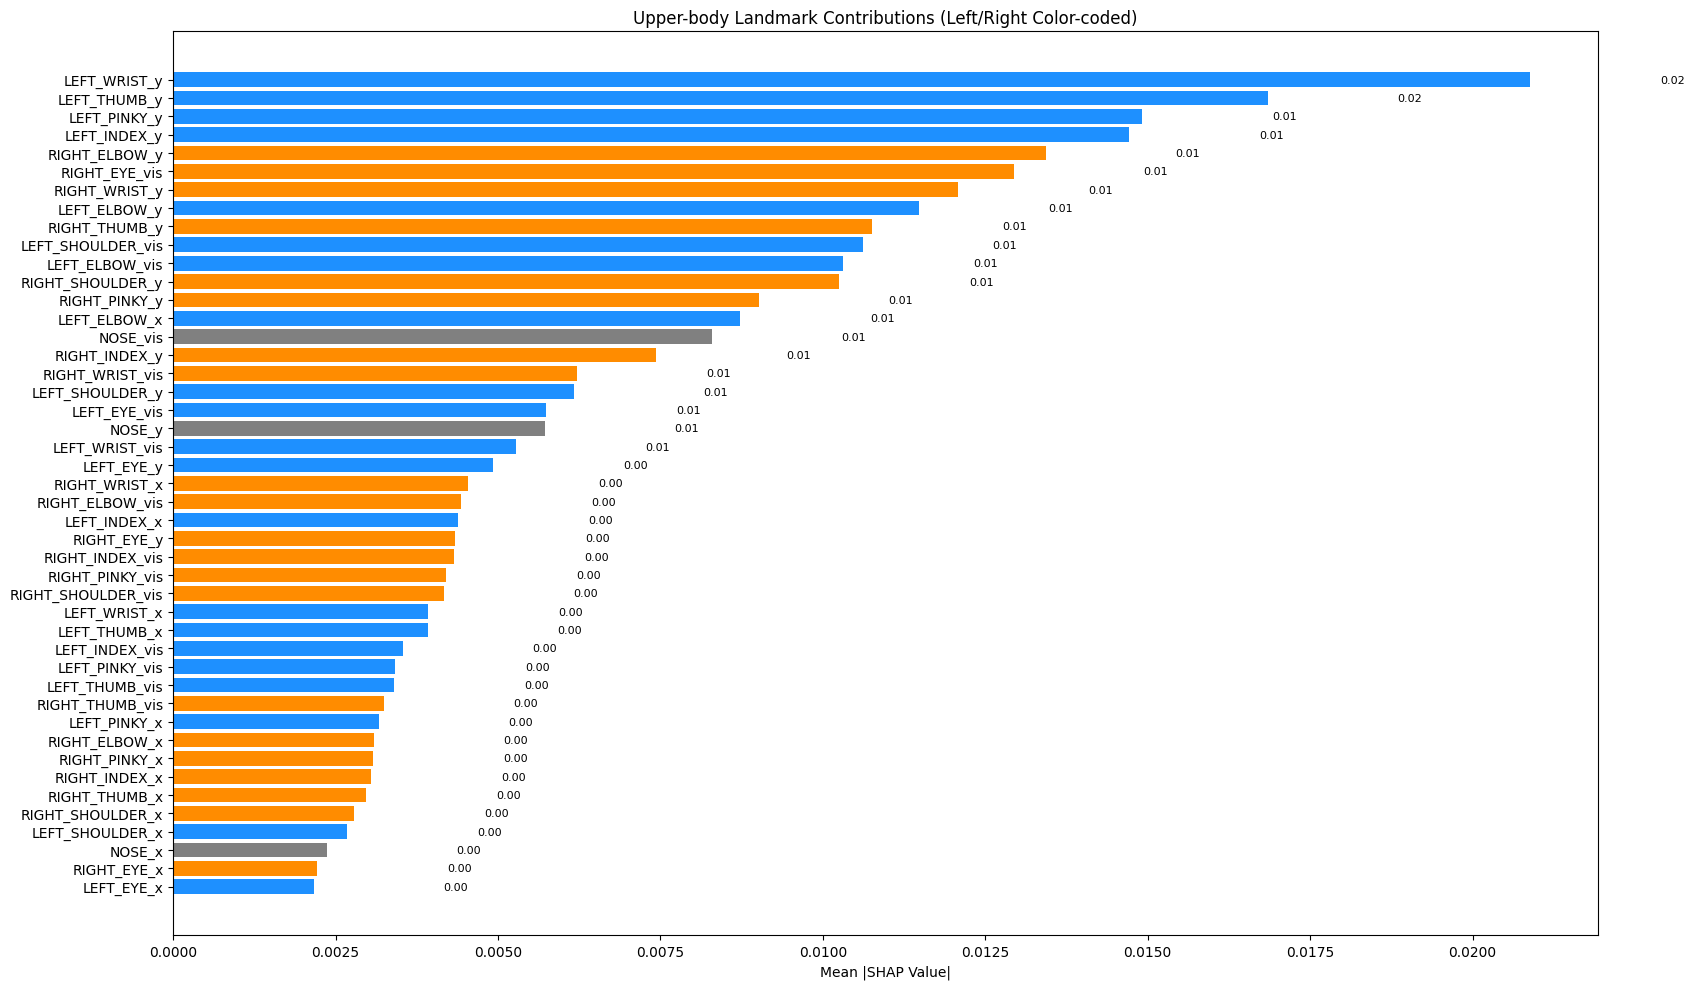
\includegraphics[width=0.8\textwidth]{image/shap_upper.png}
\caption{SHAP-based importance of upper-body pose landmarks for the Random Forest model.}
\label{fig:shap_rf}
\end{figure}

% ==============================
\subsection{APP}

A simple UI is made so that the user can upload their concerned childs video to the hompage and then upon the upload the probability of autistics behaviours is shown. There is a dedicated webpage where the user is guided on how to upload the video.


Frontend was developed using React.js framework. Backend is made with flask. Best model is dumped as *.pkl in the backend to generate prediction.

\begin{figure}[htbp]
\centering

\includegraphics[width=0.8\textwidth]{image/ui1.jpeg}
\caption{Hompage of our screening app}
\label{fig:home}
\end{figure}

In the figure \ref{fig:home}, this is a interface where user can upload centain videos of their child is suspected by clicking the upload button.

\begin{figure}[htbp]
\centering
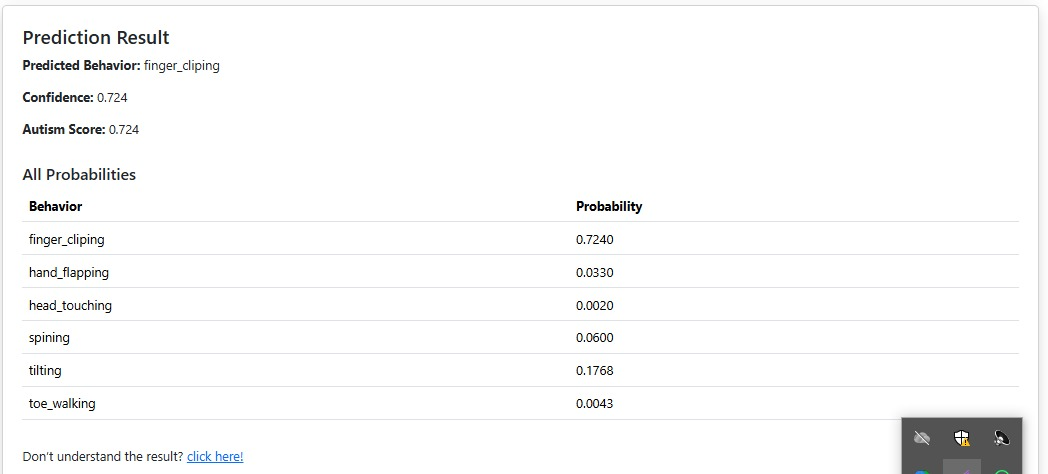
\includegraphics[width=0.8\textwidth]{image/ui2.jpeg}
\caption{App showing result after test video uploading}
\label{fig:result}
\end{figure}

Then In the figure \ref{fig:result}, this is the result shown where certain five trait possibility is shown and verdicts a final statement whether the screening from professional is needed or not.

% ==============================
\subsection{Key Findings and Discussions}


Finger clipping and hand flapping are the hardest to distinguish not because the models are weak, but because these two behaviors are naturally similar in children with autism. They often occur together, look alike in motion patterns, and share similar acceleration and rhythm signatures. No model can fully untangle what's inherently tangled.

Even so, Gradient Boosting and CNN-BiLSTM both prove capable. Gradient Boosting hits 0.96+ AUC for all five behaviors, and CNN-BiLSTM stays above 0.89. For spinning, tilting, and head touching, both models are nearly flawless.

Here's what this means practically. For a new suspected child, you don't need to rely on subjective observation alone. These models take statistical features from motion data — like acceleration peaks, rhythm consistency, and duration patterns — and add temporal dependency through architectures like BiLSTM and GRU. As a result we get an automated, objective evaluation of five core autism-related behaviors.

But we can not ignore the limitation. Because finger clipping and hand flapping are behaviorally related, confusion between them will persist. A clinician should still look closely when the model flags one but not the other — that's where real insight lives.

In the path forward, combining both models. Use Gradient Boosting for well-calibrated probability scores and CNN-BiLSTM for capturing temporal sequences. Together, they cover each other's weaknesses. For hand flapping specifically, lower the decision threshold — the AUC shows the model ranks it well, it just needs a nudge.



% ==============================
\section*{Chapter Summary}

In the foregoing chapter, the development of a pose-based system for autism behavioral classification was tried to be covered. The classification of the behavioral patterns of autism was done by comparing the conventional machine learning techniques with the BiLSTM-based temporal models. The classification was done using different metrics. The results shows that Gradient Boosting can be used as a reliable baseline for it promising log-loss while test validating and the importance of temporal information, especially for short video clips, is also emphasized. The work shows that the non invasive autism behavior analysis is possible in a scalable manner.
